\documentclass{article}
\usepackage{fullpage}

\usepackage{amsmath,cancel}
\usepackage{graphicx}
\usepackage{color}
\usepackage{alltt}
\newcommand{\red}[1]{{\color{red}#1}}
\newcommand{\cyan}[1]{{\color{cyan}#1}}
\newcommand{\blue}[1]{{\color{blue}#1}}
\newcommand{\magenta}[1]{{\color{magenta}#1}}
\newcommand{\yellow}[1]{{\color{yellow}#1}}
\newcommand{\green}[1]{{\color{green}#1}}
 
\newcommand{\bkt}[1]{\langle \mbox{ #1 } \rangle}
\newcommand{\br}{\mbox{~}|\mbox{~}}
 
\newcommand{\ns}[1]{\newpage {\bf #1}}

\setlength{\parindent}{0in}
 
\begin{document}

\LARGE 

\centerline{$T(n) = 2T(n/2) + cn$}

\hrulefill

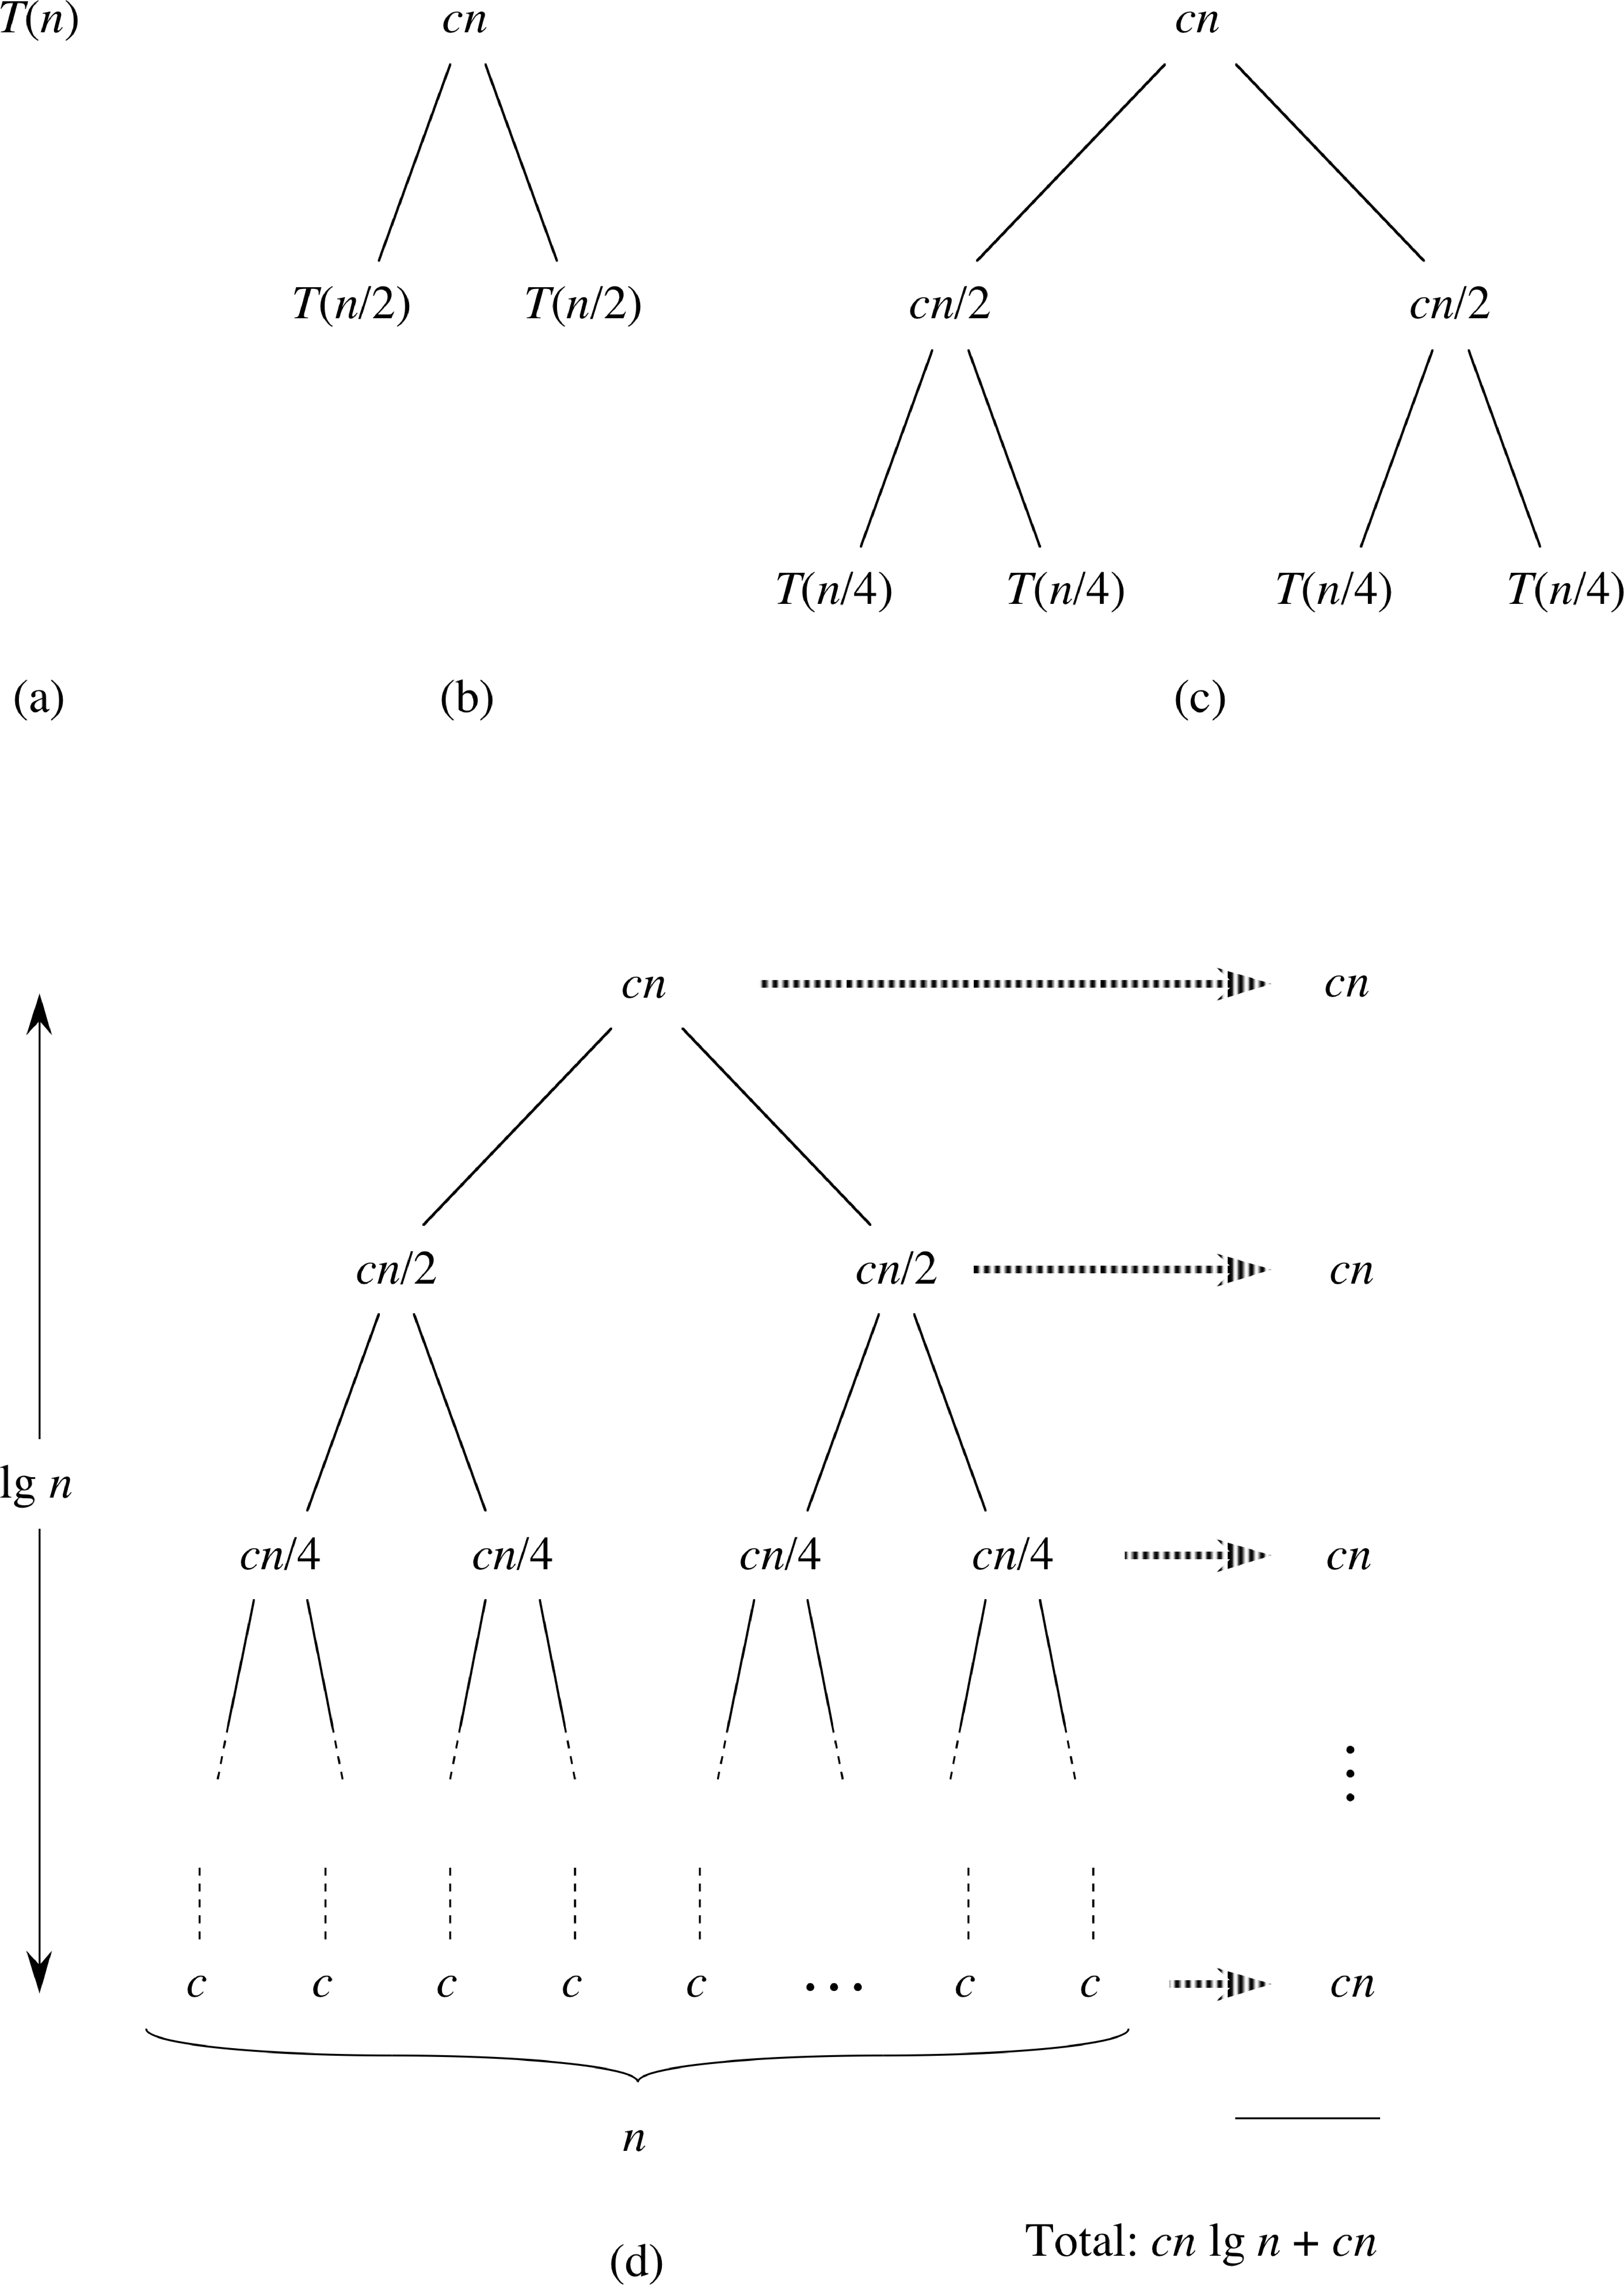
\includegraphics[width=0.85\textwidth]{Fig-2-5.pdf}


{\bf Subarray (and Mergesort) Recurrence}
\begin{align*}
  T(1) &= c\\
  T(n) &= 2T(n/2) + cn
\end{align*}

\begin{align*}
  T(n) &= \cancel{2T(n/2)} + cn\\
  \cancel{2T(n/2)} &= \cancel{2^2T(n/2^2)} + 2cn/2 \\
  \cancel{2^2T(n/2^2)} &= \cancel{2^3T(n/2^3)} + 2^2cn/2^2\\
  \cancel{2^3T(n/2^3)} &= \cancel{2^4T(n/2^4)} + 2^3cn/2^3\\
  &\ldots\\
  \cancel{2^{\lg n - 1}T(n/2^{\lg n - 1})} &= 2^{\lg n}T(1) + 2^{\lg n - 1}cn/2^{\lg n - 1}
  \end{align*}

\begin{align*}
  T(n) &=  c2^{\lg n} + \sum_{i=0}^{\lg n -1}cn\\
  &=  cn + cn\lg n\\
  &= \Theta(n \lg n)
  \end{align*}




\end{document}





